\documentclass[10pt,hyperref]{article}

\usepackage{tocloft} % http://ctan.org/pkg/tocloft
\setlength{\cftsubsecnumwidth}{4em} % Set length of number width in ToC for \subsection
\usepackage{graphicx, color, amsmath, amssymb, latexsym, float}
\usepackage{array, natbib, booktabs, multirow, rotating}

%% for helvetica
\usepackage{siunitx}
\sisetup{detect-all}
% \usepackage{helvet}
% \usepackage{sansmath}
% \sansmath

%% other mathfonts
\usepackage{fourier}
%\usepackage[sc]{mathpazo}

\usepackage{fancyhdr, setspace, perpage, longtable}
\usepackage[small,tight]{subfig}

%%--UPDATE THE pdftitle, pdfauthor, pdfsubject, and pdfkeywords fields--%%
\usepackage[
	pdftex,colorlinks=true,
	pdftitle={ Summary Report},
	pdfauthor={Paul Hobson, Geosyntec Consultants (phobson@geosyntec.com)},
	pdfkeywords={Stormwater, Stormwater monitoring, BMP, BMP monitoring, International BMP Database},
	pdfsubject={Stormwater and BMP monitoring},
	menucolor={black},
	citecolor={black},
	linkcolor={black},
	pdfpagelabels, plainpages=false]
	{hyperref}
\usepackage{fancyhdr, setspace, perpage}
%\usepackage[titles]{tocloft}
\usepackage[margin=1.1in]{geometry}

\graphicspath{{figures}{figures/statplot}{figures/scatterplot}}

\definecolor{myblue}{RGB}{0,88,176}

%\setlength{\cftbeforechapskip}{2ex}
%\setlength{\cftbeforesecskip}{0.5ex}

\pagestyle{fancy}
\fancyhead{}
\fancyfoot{}
\headheight 24pt
\textheight 8.5in
\renewcommand{\headrulewidth}{0.25pt}
\renewcommand{\footrulewidth}{0pt}
%\fancyhead[C]{Geosyntec Consultants}

%%--ADD AS SHORT TITLE FOR HEADER--%%
%\fancyhead[L]{blah}

%%--ADD YOUR OFFICE LOCATION--%%
\fancyhead[R]{}
\fancyfoot[R]{{\color{myblue}International Stormwater BMP Database}}
%\fancyhead[L]{Performance Summary for __VARTITLE in Stormwater}
\fancyhead[L]{__VARTITLE}
\fancyfoot[L]{\thepage}
%\fancyfoot[L]{\includegraphics[scale=0.3]{Geosyntec_logo_name.pdf}}
%\fancyfoot[R]{\includegraphics[scale=0.7]{Geosyntec_logo_text.pdf}}

\parindent=0in
\parskip=12pt

%%%% Document-specific commands
\newcommand{\ssu}[1]{\ensuremath{^\textrm{#1}}} %% superscript command
\newcommand{\ssd}[1]{\ensuremath{_\textrm{#1}}}%% subscript command

%% redefine upright \othermu as \mu
%%for when not using the fourier package
%\newcommand{\othermu}[1]{\mu{#1}}

\numberwithin{equation}{section}
\numberwithin{figure}{section}
\numberwithin{table}{section}

%%--ADD AUTHORS' NAMES AND COMPANY INFO--%%
\author{Prepared For: \\
		Water Environment Research Foundation \\ \vspace{4mm} \\
		Prepared By: \\
        Geosyntec Consultants, Inc. \\
        and Wright Water Engineers, Inc.}

%%--ADD DOCUMENT'S FULL TITLE--%%
\title{Categorical Summary of BMP Performance for Stormwater __VARTITLE Data \\
	   Contained in the International Stormwater BMP Database}% \\ \vspace{15mm}
	   %Stormwater and BMP Performance Database \\ \vspace{15mm}
	   % \\ \vspace{15mm}}

%%--ADD DATE OF DOCUMENT--%%
\date{\today}
\pagenumbering{roman}
\setcounter{page}{0}
\begin{document}
\maketitle
\thispagestyle{empty}
\clearpage
\tableofcontents
\clearpage
\pagenumbering{arabic}
\section[Description of Statistics]{Description of Statistics Used in this Report}
This report provides a concise statistical summary of BMP performance data
contained in the International Stormwater BMP Database.  The analysis focuses
on the distribution of effluent water quality from individual events by BMP
category, thereby providing greater weight to those BMPs for which there are a
larger number of data points reported. In other words, the performance analysis
presented in this technical summary is ``storm-weighted'', as opposed to
``BMP weighted''\footnotemark[1].

The statistical summaries have been organized by BMP and then by constituent.
For each data set, influent and effluent summary statistics are presented in a
table followed by graphical summaries.

\subsection{Tabular Summaries}
The summary tables include both parametric and non-parametric statistics.
Parametric statistics operate under the assumption that data arise from a
single statistical distribution that can be described mathematically using
coefficients, or parameters, of that distribution.  The mean and standard
deviation are example parameters of the normal, or Gaussian, distribution.
Non-parametric statistics are fundamentally based on the ranks\footnotemark[2]
of the data with no need to assume an underlying distribution.  Non-parametric
statistics do not depend on the magnitude of the data and are therefore
resistant to the occurrence of a few extreme values (i.e., high or low values
relative to other data points do not significantly alter the statistic)
\footnotemark[3].

Table ~\ref{tab:StatList} summarizes the parametric and non-parametric
statistics commonly used to describe data sets. Definitions for each summary
statistic included in the tables are provided in Table ~\ref{tab:StatDescr}.

\begin{table}[b!ht]
    \caption{Example Common Parametric and Non-Parametric Descriptive Statistics}
    \label{tab:StatList}
    \centering
    \begin{tabular}{p{1.5in} p{1.5in} p{1.5in}}
    \toprule
    \textbf{Statistic Category} & \textbf{Parametric} & \textbf{Non-Parametric} \\
    \toprule
    Measures of Location & Mean & Median \\
    \midrule
    Measures of Spread & Variance, Standard Deviation & Interquartile Range, Median Absolute Deviation \\
    \midrule
    Measures of Skew & Coefficient of Skewness & Quartile Skew Coefficient \\
    \bottomrule
    \end{tabular}
\end{table}

\footnotetext[1]{
    There are several viable approaches to evaluating the BMP Database.  Two
    general approaches that have been presented in the past (Geosyntec and WWE
    2008) are the ``BMP-weighted'' and ``storm-weighted'' approaches. The
    BMP-weighted approach represents each BMP with one value representing the
    central tendency of the BMP study, whereas the storm-weighted approach
    combines all of the storm events for the BMPs in each category and analyzes
    the overall storm-based data set. The storm-weighted approach has been
    selected for this report.
}

\footnotetext[2]{
    In this context, ranks refer to the positions of the data after being
    sorted by magnitude.
}


\footnotetext[3]{
    Helsel, D.R. and R. M. Hirsch, 2002. Statistical Methods in Water
    Resources Techniques of Water Resources Investigations, Book 4, Chapter A3.
    U.S. Geological Survey. 522 pages.
    \url{http://pubs.usgs.gov/twri/twri4a3/}
    }

\subsection{Graphical Summaries}
In addition to the summary tables provided for each BMP/constituent
combination, influent/effluent box plots and non-exceedance probability
plots are provided. Box plots (or box and whisker plots) provide a schematic
representation of the central tendency and spread of the influent and effluent
data sets. Box plots can also be used to indicate whether the influent median
is statistically different than the effluent median. A key for the box plots
is provided in Figure ~\ref{fig:bpLeg}.

Probability plots illustrate the empirical distribution of the data.  A
comparison of the influent and effluent probability plots indicates whether
there may be differences among all percentiles (not just the median) and
whether the influent and effluent data sets are similarly distributed.
Probability plots also provide a quick method of identifying the probability
that an individual sample would be less than or equal to a particular value.
For example, the effluent probability plot may be used to identify the
probability that a particular water quality threshold would be met (e.g., 40\%
chance that effluent concentration would be less than or equal to 1 mg/L). It
should be noted, however, that there is not a one-to-one correlation between
the percentiles in the influent data and the percentiles in the effluent data.
For example, the median influent concentration and the median effluent
concentrations may not occur in the EMC samples collected during the same
storm. Although the influent and effluent concentrations in a probability plot
are not paired values, the relative position and slope of the two populations
are a good indication of the effectiveness of the BMP. When generating the
probability plots, the detection limits were used for non-detect values (i.e.,
ROS estimates or half the DL were not used).  Non-detects are depicted as
triangles pointing down for influent data and pointing up for effluent data.

Influent vs. effluent scatterplots depict paired data to provide an indication
of how effluent concentrations may be related to the influent concentrations.
Data points below the 45 degree line indicate removals whereas data points
above the 45 degree line indicate increases.  Detection limits are shown for
non-detect values. If both the influent and effluent are non-detect, then a
diamond symbol is used.  If only the effluent is non-detect then a triangle
symbol pointing up is used.  If only the influent is non-detect, then a
triangle symbol pointing down is used.

\begin{longtable}[pt]{p{1.5in} p{4in}}
    \caption{Common Parametric and Non-Parametric Descriptive Statistics}
    \label{tab:StatDescr} \\

    % header for first page of table
    \toprule
    \multicolumn{1}{c}{\textbf{Statistic}} &
    \multicolumn{1}{c}{\textbf{Definition/Description}} \\
    \toprule
    \endfirsthead

    % header for all subsequent pages of table
    \multicolumn{2}{c}{{
        \tablename\ \thetable{} -- continued from previous page
    }} \\

    \toprule
    \multicolumn{1}{c}{\textbf{Statistic}} &
    \multicolumn{1}{c}{\textbf{Definition/Description}} \\
    \toprule
    \endhead

    % footer for 1st thru (n-1)th page of table
    \multicolumn{2}{r}{{Continued on next page}} \\
    \endfoot

    % footer for last (nth) page of table
    \bottomrule
    \endlastfoot

    Count & Total number of data points analyzed.  Most BMP data sets include
    only event mean concentrations (EMCs).  The exception includes BMPs with
    permanent pools (retention ponds and wetland basins) where grab samples
    were also included.  \\

    \midrule
    Number of Non-detects & The number of censored values that were reported
    below the analytical detection limits. Laboratory estimated values (i.e.,
    ``J'' values) were treated as detected values. The plotting position, or
    regression-on-order statistics (ROS), method described in Helsel and Cohn
    (1988)\footnotemark[4] was used to estimate censored values using the
    distribution of uncensored values for each study.   \\

    \midrule
    Mean (95\% conf. interval) & The mean of the data points and the 95\%
    confidence interval (CI) about the mean.  Provides a parametric measure of
    the central tendency. The confidence interval was computed using the
    bias-corrected and accelerated (BCa) bootstrap method described by
    Efron and Tibishirani (1993)\footnotemark[5].\\

    \midrule
    Std. Dev. & The standard deviation of the data points. \\

    \midrule
    Coeff. of Variation & The ratio of the standard deviation to the absolute
    value of the mean. \\

    \midrule
    Skewness & The coefficient of skewness of the data points.  \\

    \midrule
    Median (95\% conf. interval)  & The median of the data points and the 95\%
    confidence interval (CI) about the median. The confidence interval was
    computed using the bias corrected and accelerated (BCa) bootstrap method
    described by Efron and Tibishirani (1993)\footnotemark[5].   \\

    \midrule
    $25^{\mathrm{th}}$ and $75{\mathrm{th}}$ percentiles & The difference
    between the 25th and 75th percentiles is the inter-quartile range, which is
    a non-parametric measure of the spread of the data.  \\

    \midrule
    Number of paired data & The number of storm events where influent and
    effluent samples were simultaneously collected.\\

    \midrule
    Wilcoxon p-value & The statistical significance value for the signed-rank
    test, which is based on the alternative hypothesis that the median of the
    paired influent/effluent differences is not equal to zero.  This
    non-parametric test applies only to paired data sets and is performed on
    log-transformed data (base 10) to improve the symmetry of the distribution
    of the differences between the data pairs.  A p-value less than 0.05
    indicates that the influent and effluent concentrations are statistically
    significantly different at the 95\% confidence level. \\

    \midrule
    Mann-Whitney p-value & The statistical significance value for the rank-sum
    test, which is based on the alternative hypothesis that the influent and
    effluent medians differ. This non-parametric test applies to two
    independent data sets.  A p-value less than 0.05 indicates that the
    influent and effluent median concentrations are statistically significantly
    different at the 95\% confidence level.\\

    % \midrule
    % p-values, detects (normal, log-normal) & Shapiro-Wilk goodness-of-fit
    % p-values for testing the null hypothesis that the data (or log of the data)
    % arise from the normal distribution.  A p-value greater than 0.05 indicates
    % the null hypothesis cannot be rejected at the 95\% confidence level.
    % A p-value less than 0.05 indicates the null hypothesis can be rejected at
    % the 95\% confidence level.  The test was only applied to the detected
    % values in their original units as well as the log of the values.  The
    % former tests whether the data arise from normal distribution whereas the
    % latter tests whether the data arise from the log-normal distribution. \\
\end{longtable}

\footnotetext[4]{
    Helsel, D.R. and T. A. Cohn (1988).  ``Estimation of descriptive statistics
    for multiply censored water quality data'', \textit{Wat. Resour. Res.}
    24, 1997-2004.
}

\footnotetext[5]{
    Efron, B. and R. Tibishirani (1993). \textit{An Introduction to the
    Bootstrap}. Chapman \& Hall, New York.
}


\begin{figure}[t!]
    \centering
    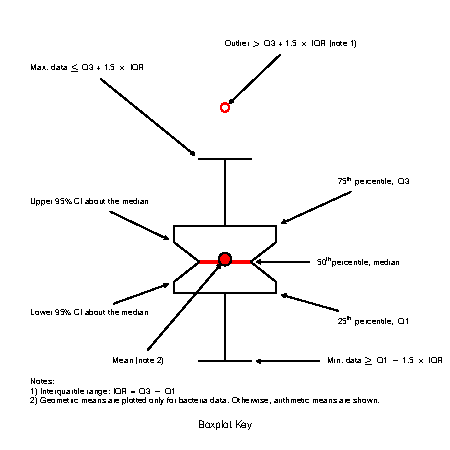
\includegraphics[scale=1.25]{figures/boxplotlegend.pdf}
    \caption{Graphical explanation of box and whisker plots}
    \label{fig:bpLeg}
\end{figure}
\clearpage


